% !TEX root = task-3-17-4.tex
% Editable task bank. Append new BankTask blocks at the end of the document.
\documentclass[12pt,a4paper]{article}
\usepackage{physics-textbook}
\usepackage{graphicx,needspace}
\usetikzlibrary{decorations.pathmorphing}
\newif\ifShowSolutions
\ifdefined\TutorEdition
  \ShowSolutionstrue
\else
  \ShowSolutionsfalse % Change to \ShowSolutionstrue to display solutions.
\fi
\newcounter{banktask}
\newsavebox{\BankTaskBox}
\newcommand{\BankTaskContent}[3]{%
  \noindent\textbf{\thebanktask.}\quad #2\par
  \ifShowSolutions
    \Needspace{50mm}% Keep the solution heading with its opening text or diagram.
    #3\par
    \ifdefined\TutorEdition
      \ifcsname TutorSource#1\endcsname
        \nopagebreak\smallskip{\small\csname TutorSource#1\endcsname\par}%
      \fi
    \fi
  \fi
}
\newcommand{\BankTask}[3]{%
  \refstepcounter{banktask}\par\medskip
  \sbox{\BankTaskBox}{\begin{minipage}{\linewidth}%
    \BankTaskContent{#1}{#2}{#3}\end{minipage}}%
  \ifdim\dimexpr\ht\BankTaskBox+\dp\BankTaskBox\relax>\dimexpr\textheight-20mm\relax
    \Needspace{35mm}\BankTaskContent{#1}{#2}{#3}%
  \else
    \Needspace{\dimexpr\ht\BankTaskBox+\dp\BankTaskBox\relax}%
    \noindent\usebox{\BankTaskBox}\par
  \fi
  \medskip
}
\begin{document}
\BookSubsection{3.17.4}{Магнитное поле прямого провода с током}


% Source 33064: https://phys-ege.sdamgia.ru/problem?id=33064
\BankTask{33064}{
Три параллельных длинных прямых проводника $1$, $2$ и $3$ расположены на одинаковом расстоянии а друг от друга (см. рис. а и б). В каждом проводнике протекает электрический ток силой I. Токи во всех проводниках текут в одном направлении. Определите направление результирующей силы, действующей на проводник $1$ со стороны проводников $2$ и $3$. Сделайте рисунок, указав в области проводника $1$ векторы магнитной индукции полей, созданных проводниками $2$ и $3$, вектор магнитной индукции результирующего магнитного поля и вектор результирующей силы. Ответ поясните, опираясь на законы электродинамики.

\begin{center}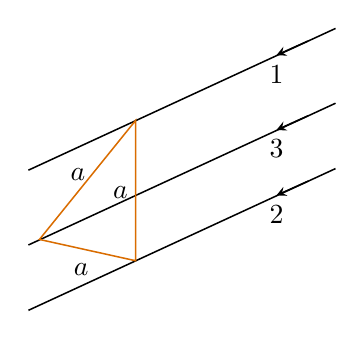
\begin{tikzpicture}[>=stealth,line width=.55pt]\draw(-.5,0)--(3.4,1.8) (-.5,.83)--(3.4,2.63) (-.5,1.78)--(3.4,3.58);\draw[orange!85!black](.86,.63)--(.86,2.41)--(-.36,.9)--cycle;\foreach \y/\i in {0/2,.83/3,1.78/1}{\draw[->](3.05,\y+1.64)--(2.65,\y+1.46)node[below]{$\i$};}\node at(.67,1.49){$a$};\node at(.13,1.73){$a$};\node at(.17,.52){$a$};\end{tikzpicture}\end{center}
Рис. а)

\begin{center}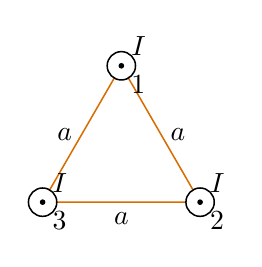
\begin{tikzpicture}[>=stealth,line width=.55pt]\draw[orange!85!black](0,0)--(2,0)--(1,1.732)--cycle;\foreach \x/\y/\i in {0/0/3,2/0/2,1/1.732/1}{\draw[fill=white](\x,\y)circle(.18);\fill(\x,\y)circle(.036);\node[below right]at(\x,\y){$\i$};\node[above right]at(\x,\y){$I$};}\node[below]at(1,0){$a$};\node[left]at(.5,.86){$a$};\node[right]at(1.5,.86){$a$};\end{tikzpicture}\end{center}
Рис. б)
}{
\smallskip\noindent\textbf{Решение}\par
На проводник $1$ со стороны проводников $2$ и $3$ действует результирующая сила, направленная вниз (см. рис.).
\begin{center}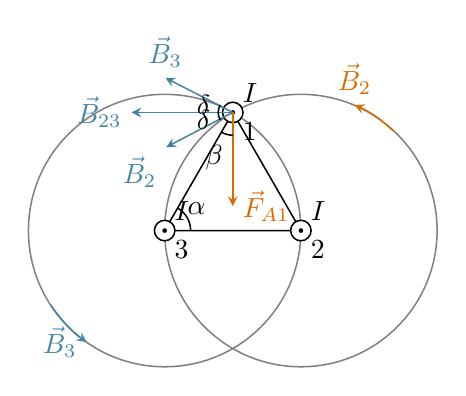
\begin{tikzpicture}[>=stealth,line width=.55pt]\draw[gray](0,0)circle(1.73) (1.73,0)circle(1.73);\draw(0,0)--(.865,1.5)--(1.73,0)--cycle;\foreach \x/\y/\i in {0/0/3,1.73/0/2,.865/1.5/1}{\draw[fill=white](\x,\y)circle(.13);\fill(\x,\y)circle(.03);\node[below right]at(\x,\y){$\i$};\node[above right]at(\x,\y){$I$};}\draw[->,cyan!60!black](.865,1.5)--(.01,1.94)node[above]{$\vec B_3$};\draw[->,cyan!60!black](.865,1.5)--(.02,1.06)node[below left]{$\vec B_2$};\draw[->,cyan!60!black](.865,1.5)--(-.42,1.5)node[left]{$\vec B_{23}$};\draw[->,orange!85!black](.865,1.5)--(.865,.31)node[right]{$\vec F_{A1}$};\draw[->,orange!85!black](2.91,1.26)arc(46:66:1.73)node[above]{$\vec B_2$};\draw[->,cyan!60!black](-1.45,-.94)arc(213:235:1.73)node[left]{$\vec B_3$};\draw(.68,1.5)arc(180:211:.185)node[left]{$\delta$};\draw(.68,1.5)arc(180:149:.185)node[left]{$\delta$};\draw(.33,0)arc(0:60:.33)node[right]{$\alpha$};\draw(.72,1.25)arc(240:270:.29)node[below left]{$\beta$};\end{tikzpicture}\end{center}
Вокруг проводников $2$ и $3$ возникает магнитное поле, линии индукции которого являются окружностями. Направление линий индукции магнитного поля определяется правилом буравчика. Вектор магнитной индукции результирующего поля в области проводника $1$ определяется принципом суперпозиции полей $\vec{B}_23=\vec{B}_2 + \vec{B}_3, \,\text{где}$ $\vec{B}_2$ и $\vec{B}_3$ − векторы индукции магнитных полей, созданных проводниками $2$ и Поскольку проводник $1$ находится на одинаковом расстоянии a от каждого из проводников $2$ и $3$, по проводникам протекают токи одинаковой силы, то $|\vec{B}_2|=|\vec{B}_3|=B.$
Из геометрических построений видно, что угол между векторами $\vec{B}_2$ и $\vec{B}_3$ составляет $60$°, значит, $\,\text{дельта} =30 ^\circ .$ Следовательно, вектор магнитной индукции $\vec{B}_23$ направлен горизонтально влево. Со стороны результирующего поля на проводник $1\,\text{с}$ током действует сила Ампера F$_{A1}$, направление которой определяется правилом левой руки. Таким образом, результирующая сила, действующая на проводник $1$ со стороны проводников $2$ и $3$, направлена вертикально вниз.

Ответ: на проводник $1$ со стороны проводников $2$ и $3$ действует результирующая сила, направленная вниз.
}

\end{document}
